\documentclass[11pt]{penrose}


\usepackage{mathsphystools}

\author{Rashid M. Talha}

\newenvironment{problem}[2][Question]{\textbf{#1 #2.}\par}{}
\newcommand{\solution}{\textit{Solution.}\hspace{2mm}}

\newcommand{\warningtext}{\textbf{Disclaimer:} Use at your own risk. Errors possible.}

\usepackage{tikz}
\usetikzlibrary{positioning, arrows}

\title{Past Paper: Mathematical Modelling}
\subtitle{Midterm Exam, 2024}
\begin{document}

\maketitle
\warningtext

\begin{problem}{1}
    Let $a_{n}$ be the annuity after $n$ months, $b$ be the monthly deposit amount and $r$ be the monthly rate of change. The given situation can be modelled by the first order linear recurrence relation $a_{n+1} = r a_{n} + b$ with the solution
    \begin{equation*}
        a_{k} = r^{k} c + \frac{b}{1-r},
    \end{equation*}
    and the equilibrium value (obtained by setting $a_{n+1} = a_{n} = \bar{a}$)
    \begin{equation*}
        a_{n+1} = r a_{n} + b
        \implies
        \bar{a} = r \bar{a} + b
        \implies
        \bar{a} = \frac{b}{1 - r}.
    \end{equation*}
    In the present case, $r = 1.01$ and $b = -1000$.

    So, the equilibrium value is $\bar{a} = \$ 100,000$ and the solution is $a_{n} = 100000 - 50000 (1.01)^{n}$.

    The equilibrium value shows that if the initial deposit is $\$ 100,000$ then the net value of the annuity will remain the same each month. An initial value less than this amount will eventually deplete, while a larger initial value will continue to increase.

    Now, $a_{n} = 0$ corresponds to $-50000 (1.01)^{n} + 100000 = 0 \implies (1.01)^{n} = 2$. Therefore,
    \begin{equation*}
        n = \frac{ \ln{2} }{ \ln{1.01} } = 69.660\dots.
    \end{equation*}
    Consequently, the annuity will deplete after $70$ months.
\end{problem}

\begin{problem}{2}
    Let $P = P_{n} = P_{n+1}$ and $Q = Q_{n} = Q_{n+1}$ be the equilibrium values of price and quantity, respectively. Then,
    \begin{equation*}
        \begin{aligned}
            P_{n+1} &= P_{n} - 0.1(Q_{n} - 500)\\
            Q_{n+1} &= Q_{n} + 0.2(P_{n} - 100)
        \end{aligned}
        \implies
        \begin{aligned}
            P &= P - 0.1(Q - 500)\\
            Q &= Q + 0.2(P - 100)
        \end{aligned}
        \implies
        \begin{aligned}
            Q &= 500 \\ P &= 100
        \end{aligned}
    \end{equation*}

    Numerical results (4 iterations) for the two given cases are:

    \begin{tabularx}{0.42\textwidth}{D{10mm}CC}
        \toprule
        $n$ & $P_{n}$ & $Q_{n}$ \\
        \midrule
        $0$ & $200$ & $500$ \\
        $1$ & $200$ & $520$ \\
        $2$ & $198$ & $540$ \\
        $3$ & $194$ & $559.6$ \\
        $4$ & $188.04$ & $578.4$ \\
        \bottomrule
    \end{tabularx}
    \hfill
    \begin{tabularx}{0.42\textwidth}{D{10mm}CC}
        \toprule
        $n$ & $P_{n}$ & $Q_{n}$ \\
        \midrule
        $0$ & $100$ & $600$ \\
        $1$ & $90$ & $600$ \\
        $2$ & $80$ & $598$ \\
        $3$ & $70.2$ & $594$ \\
        $4$ & $60.8$ & $588.04$ \\
        \bottomrule
    \end{tabularx}
\end{problem}

\clearpage
\begin{problem}{3}
    \underline{Method:} Let $\lambda = 0$. Consider any path from $A$ to $F$ such that every edge along that path has a positive capacity. Subtract the lowest edge capacity from every edge along this path, and add this number to $\lambda$. Repeat this process until no valid path is left. Then, $\lambda$ is the maximum flow through the network.

    \underline{Solution:}
    \begin{itemize}
        \item Take $A \to B \to D \to F$. The minimum available edge capacity is $2$. Subtract this from $8, 2$ and $10$ (edge capacities on $A \to B$, $B \to D$ and $D \to F$, respectively).
        \item Take $A \to C \to E \to F$. The minimum available edge capacity is $8$. Subtract this from $10, 12$ and $8$ (edge capacities on $A \to C$, $C \to E$ and $E \to F$, respectively).
        \item Take $A \to B \to E \to D \to F$. The minimum available edge capacity is $4$. Subtract this from $6, 7, 4$ and $8$ (edge capacities on $A \to B$, $B \to E$, $E \to D$ and $D \to F$, respectively).
    \end{itemize}
    No other valid paths (where every edge has a positive capacity) are possible. So, the maximum flow is $2 + 8 + 4 = 14$. The state of the network after each operation is:

    \begin{equation*}
    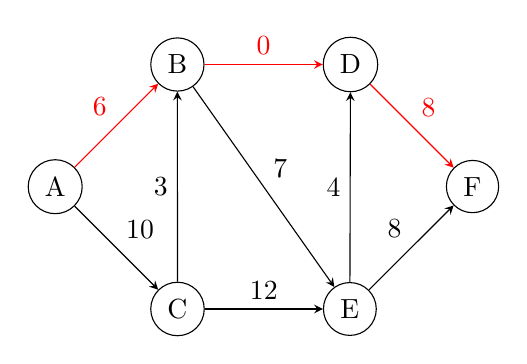
\begin{tikzpicture}[->, >=stealth, node distance=1.5cm, auto, scale=1, transform shape]
        \node (A) [circle, draw] {A};
        \node (B) [circle, draw, above right=of A] {B};
        \node (C) [circle, draw, below right=of A] {C};
        \node (D) [circle, draw, right=of B] {D};
        \node (E) [circle, draw, right=of C] {E};
        \node (F) [circle, draw, below right=of D] {F};

        \path
            (A) edge[red] node {6} (B)
            (A) edge node {10} (C)
            (B) edge[red] node {0} (D)
            (C) edge node {3} (B)
            (C) edge node {12} (E)
            (B) edge node {7} (E)
            (D) edge[red] node {8} (F)
            (E) edge node {4} (D)
            (E) edge node {8} (F);
    \end{tikzpicture}
    \end{equation*}
    \begin{equation*}
    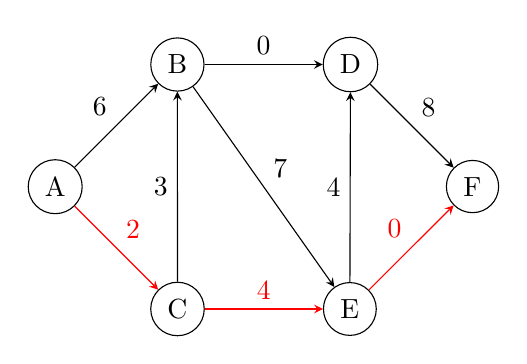
\begin{tikzpicture}[->, >=stealth, node distance=1.5cm, auto, scale=1, transform shape]
        \node (A) [circle, draw] {A};
        \node (B) [circle, draw, above right=of A] {B};
        \node (C) [circle, draw, below right=of A] {C};
        \node (D) [circle, draw, right=of B] {D};
        \node (E) [circle, draw, right=of C] {E};
        \node (F) [circle, draw, below right=of D] {F};

        \path
            (A) edge node {6} (B)
            (A) edge[red] node {2} (C)
            (B) edge node {0} (D)
            (C) edge node {3} (B)
            (C) edge[red] node {4} (E)
            (B) edge node {7} (E)
            (D) edge node {8} (F)
            (E) edge node {4} (D)
            (E) edge[red] node {0} (F);
    \end{tikzpicture}
    \end{equation*}
    \begin{equation*}
    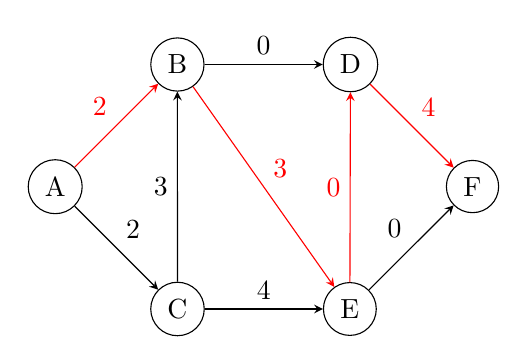
\begin{tikzpicture}[->, >=stealth, node distance=1.5cm, auto, scale=1, transform shape]
        \node (A) [circle, draw] {A};
        \node (B) [circle, draw, above right=of A] {B};
        \node (C) [circle, draw, below right=of A] {C};
        \node (D) [circle, draw, right=of B] {D};
        \node (E) [circle, draw, right=of C] {E};
        \node (F) [circle, draw, below right=of D] {F};

        \path
            (A) edge[red] node {2} (B)
            (A) edge node {2} (C)
            (B) edge node {0} (D)
            (C) edge node {3} (B)
            (C) edge node {4} (E)
            (B) edge[red] node {3} (E)
            (D) edge[red] node {4} (F)
            (E) edge[red] node {0} (D)
            (E) edge node {0} (F);
    \end{tikzpicture}
    \end{equation*}
\end{problem}

\clearpage
\begin{problem}{4}
    The given ODE is $X'(t) = k X (N - X)$ with $k > 0$ and $X(t_{0}) = X_{0}$. This is a separable equation. So, separating $X$ and $t$ terms and decomposing into partial fractions gives
    \begin{equation*}
        \int \frac{1}{X (N-X)} \,dx = \int k \,dt
        \implies \int \paren*{\frac{1}{X} + \frac{1}{N-X}} \,dx = \int kN \,dt
    \end{equation*}
    Upon integration, this becomes $\ln{\abs{X}} - \ln\abs{N-X} = kNt + \ln A$, where $A$ is an arbitrary constant. We simplify this further to get
    \begin{equation*}
        \frac{X}{N-X} = A e^{kNt}
        \implies
        X = \frac{N A e^{kNt}}{1 + A e^{kNt}}
        \implies
        X = \frac{N A}{A + e^{-kNt}}
    \end{equation*}
    The initial condition $X(t_{0}) = X_{0}$ leads to $A = X_{0} e^{-kNt_{0}} / (N - X_{0})$. Overall,
    \begin{equation*}
        X(t) = \frac{N A}{A + e^{-kNt}}
        \quad\text{with}\quad
        A = \frac{X_{0}}{N - X_{0}} e^{-kNt_{0}}.
    \end{equation*}
    As $t \to \infty$, $e^{-kNt} \to 0$, which means $X \to N$.

    By plotting the given data for $\ln\abs{X/(N-X)}$ against $t$ we obtain a straight line graph with gradient $0.5$ and $y$-intercept $-1.5$. Therefore, $\ln\abs{X/(N-X)} = 0.5 t - 1.5$. Now, comparing it with
    \begin{equation*}
        \ln A
        = \ln \paren*{ \frac{X_{0}}{N - X_{0}} e^{-kNt_{0}} }
        = -kNt_{0} + \ln \paren*{ \frac{X_{0}}{N - X_{0}} }
    \end{equation*}
    gives $\ln A = -1.5 \implies A = 0.223$ and $kN = 0.5 \implies k = 0.0001$, since $N = 5000$.

    Consequently,
    \begin{equation*}
        X(t = 12)
        = \frac{5000 \times 0.223}{0.223 + e^{-(0.5 \times 12)}}
        = 4945.
    \end{equation*}

    Suppose the time taken for half of the population to become infected is $t^{*}$. Then,
    \begin{equation*}
        \frac{N}{2} = \frac{N A}{A + e^{-kNt^{*}}}
        \implies
        2 = \frac{A + e^{-kNt^{*}}}{A}
        \implies
        A = e^{-kNt^{*}}.
    \end{equation*}
    Therefore,
    \begin{equation*}
        t^{*}
        = - \frac{1}{kN} \ln A
        = - \frac{1}{kN} \bparen*{ -kNt_{0} + \ln \paren*{ \frac{X_{0}}{N - X_{0}} } }
        = t_{0} - \frac{1}{kN} \ln \paren*{ \frac{X_{0}}{N - X_{0}} }.
    \end{equation*}
\end{problem}

\end{document}